\section{Pixelar}
Este filtro consiste en tomar bloques de 2x2 píxeles y asignarles a estos el promedio del bloque. De esta manera se disminuye la cálidad de la imágen.
\subsection{Código C}
	El código de C consiste en recorrer la imagen de a dos filas y dos columnas por iteración. En cada iteración se calcula el promedio de los canales de los píxeles.
	A continuación adjuntamos el pseudocódigo.

\begin{algorithm}[h!]
\caption{Promedio}
\begin{algorithmic}
  \Function{promedio}{$a :unsigned char, b: unsigned char, c: unsigned char, d: unsigned char$}  $\to \texttt{float}$
	\State float af $\gets$ a
	\State float bf $\gets$ b
	\State float cf $\gets$ c
	\State float df $\gets$ d
	return (af/4+bf/4+cf/4+df/4)
	
\EndFunction
\end{algorithmic} 
\end{algorithm}	
	
	\begin{algorithm}[h!]
\caption{Pixelar}
\begin{algorithmic}
  \Function{pixelar}{src: *unsigned char, dst: *unsigned char, cols: int, filas: int, srcRowSize: int, dstRowSize: int}
	\State $unsigned~ char~ (*srcMatrix)[srcRowSize] = (unsigned~ char (*)[srcRowSize])~ src$
	\State $unsigned~ char~ (*dstMatrix)[dstRowSize] = (unsigned~ char (*)[dstRowSize])~ dst$
	
	\For{$f \gets 0~..~filas-1; f+=2$}
		\For{$c \gets 0~..~cols-1; c+=2$}
			\State $bgra_t* p_s1 \gets (bgra_t*)$ \& $srcMatrix[f][c * 4]$
			\State $bgra_t *p_d1 \gets (bgra_t*)$ \&$dstMatrix[f][c * 4]$
			
			\State $bgra_t* p_s2 \gets (bgra_t*)$ \& $srcMatrix[f+1][c * 4]$
			\State $bgra_t *p_d2 \gets (bgra_t*)$ \&$dstMatrix[f+1][c * 4]$
			
			\State $bgra_t* p_s3 \gets (bgra_t*)$ \& $srcMatrix[f+1][(c+1) * 4]$
			\State $bgra_t *p_d3 \gets (bgra_t*)$ \&$dstMatrix[f+1][(c+1) * 4]$
			
			\State $bgra_t* p_s4 \gets (bgra_t*)$ \& $srcMatrix[f][(c+1) * 4]$
			\State $bgra_t *p_d4 \gets (bgra_t*)$ \&$dstMatrix[f][(c+1) * 4]$
			
			\State k $\gets$ 0.5
			
			\State b $\gets$ promedio(p_s$\rightarrow$b,p_s2$\rightarrow$b,p_s3$\rightarrow$b,p_s4$\rightarrow$b)
			\State g $\gets$ promedio(p_s$\rightarrow$g,p_s2$\rightarrow$g,p_s3$\rightarrow$g,p_s4$\rightarrow$g)
			\State r $\gets$ promedio(p_s$\rightarrow$r,p_s2$\rightarrow$r,p_s3$\rightarrow$r,p_s4$\rightarrow$r)
			\State a $\gets$ promedio(p_s$\rightarrow$a,p_s2$\rightarrow$a,p_s3$\rightarrow$a,p_s4$\rightarrow$a)
				
			\For{$i \gets 1~..~4$}
				\State ($p_di \rightarrow$b) $\gets$ b
				\State ($p_di \rightarrow$g) $\gets$ g
				\State ($p_di \rightarrow$r) $\gets$ r
				\State ($p_di \rightarrow$ a) $\gets$ a
				
			
		\EndFor
	\EndFor
\EndFunction

\end{algorithmic} 
\end{algorithm}
\subsection{Código ASM}
	
	
	
\subsection{Experimentación}
\subsubsection{Idea}	
	Comparamos la eficacia del código en ASM contra C y C optimizado.
	
\subsubsection{Resultados}
	\begin{figure}[h!]
	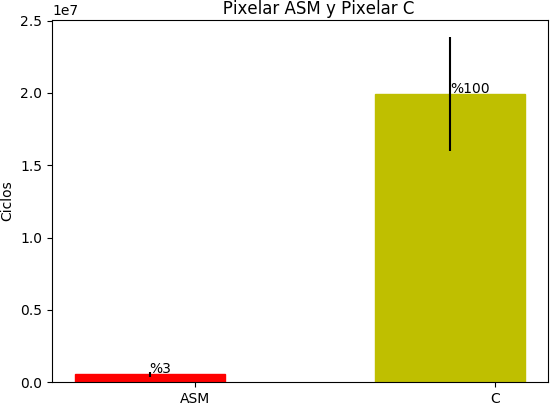
\includegraphics[width = 15 cm, height = 10 cm]{imagenes/ASMvsCPixelar.png}
\end{figure}